\section{Motivation}
Tropical cyclones are some of the most powerful and destructive weather 
systems on earth having the potential to cause major devastation and significant 
loss of life. Yet traditional global weather and climate models typically have coarse 
grid resolutions that cannot resolve the extreme pressure gradients, high wind 
speeds, and other small-scale (1-10 km) processes that drive these cyclones. The 
development of Adaptive Mesh Refinement (AMR) techniques offers a 
transformative new approach to incorporate these scales within atmospheric 
General Circulation Models (GCMs). GCMs with AMR capabilities will be able to 
identify traveling salient features and selectively enhance the grid resolution over 
them while keeping less active regions at coarser mesh spacings, thereby reducing 
computational costs. This has the potential to improve the representation of TCs 
and other extreme weather and climate events by allowing next-generation models 
to achieve unprecedented high resolutions in local areas.

\section{General circulation models}
General circulation models (GCMs) are the backbone of today's global climate 
modeling research; these models use numerical approximations to simulate the circulation 
of the Earth's atmosphere. GCMs are comprised of two components. The dynamical 
core component is considered the engine of a GCM. The atmosphere is spatially 
discretized onto a grid and the dynamical core (dycore) uses numerical methods 
to resolve the fluid motion and thermodynamic quantities on each grid. The 
second component contains the physics parameterizations. These approximate the 
atmospheric features including radiation and sub-grid scale process like convection, 
clouds, and turbulence that are not resolvable by the dycore. GCMs are used 
in wide ranging temporal scales, from hours and days for short term weather 
prediction to decades and centuries for long-term climate assessments.  

\section{High resolution in climate and weather models}
Atmospheric phenomena which have an outsized effect on humans 
and society, such as tropical cyclones, atmospheric rivers, and severe thunderstorms,
 exist on relative small spatial scales.
Even large scale global phenomena, like the Madden-Julian Oscillation, rely on
key processes like cloud formation and convection that need to be parameterized 
for resolutions higher than a few kilometers.
Decreasing the distance between grid elements improves the ability of the model
to directly resolve atmospheric features at smaller spatial scales.
Increased resolution results in broad improvements for resolving key 
climate and weather features as models can better capture physical 
processes and interactions between the atmosphere and land or ocean 
\citep{prodhomme2016benefits}. 
Increased resolution, however, is computationally intensive. The processing power and 
memory constraints of computers used
to run the models are the limiting factors in increasing horizontal resolution. Increasing resolution
not only increases the number of grid cells of the model but also requires a shorter
time step due to a more restrictive Courant-Friedrichs-Lewy (CFL) condition. As a result, a doubling of the 
horizontal resolution generally results in eight-fold more calculations.

The global climate models used in the Fifth Assessment Report by the 
Intergovernmental Panel on Climate Change (IPCC) used grid
resolutions between 50 and 300 km \citep{flato2013evaluation}. 
For comparison the average tropical cyclone has a diameter of $\sim 600$ km 
with the average cyclone eye $\sim 30$ km across. The latest
high-resolution global climate models can implement 10 - 50 km grid 
spacing \citep{kinter:13,hayhoe2017climate}. However, they are computationally 
expensive to run extensively, and they are still unable to explicitly represent key 
processes, such as clouds. The global weather models used by the European 
Centre for Medium-Range Weather Forecasts (ECMWF) and NOAA have grid 
spacings of 9 km and 13 km respectively \citep{haiden2016evaluation,dias2018equatorial}
and are only run for spans of a few weeks.
A few non-hydrostatic, partly cloud-resolving global simulations by \cite{putman:11} 
and \cite{miyamoto:13} were run for short, multi-day time periods with grid spacings in 
the $0.9 � 3.5$ km range. These simulations were single runs demonstrating the concept 
of such models and are not feasible for climate simulations or even 
numerical weather predictions. With global high-resolution GCMs burdened by 
computational costs, alternative methods are needed to increase
resolution over specific areas of interests. 

Limited area models (LAM) are one possible solution. They can operate with increased 
resolution down to $10-50$ km grid spacing for climate simulations and 1 to 3 km 
grid spacing for short-term weather forecasting. LAMs eliminate computational expense 
by numerically simulating only a small specific region (e.g the continental United States), but
this requires the lateral boundaries to be externally forced. These
boundary conditions are typically derived from coarser GCMs, which use different 
numerical schemes and physical parameterizations, thereby introducing possible biases 
or numerical discrepancies. Since LAMs are not global in scale,
key conservation properties are not obeyed. Due to these boundary conditions, 
LAMs might not be able to effectively capture the large-scale, global climate feedbacks 
triggered by localized phenomena such as tropical cyclones.


\section{Variable Resolution models}
  We are interested in combining the localized high-resolution and computational economy of LAMs with
  the numerical and physical consistency of a global model. Variable resolution 
  GCMs (VRGCMs) place additional grid elements only where high-resolution
  is required. They maintain global connectivity between the areas of coarse and fine grids cells, 
  eliminating the need for forced lateral 
  boundary conditions. In addition, they maintain two-way interactions, unlike one-way nested LAMs,
  which permit features within the refined nest to affect the global solution. VRGCM is
  a classification that encompasses any global model which implements multiple grid resolutions with
  two-way interactions. The two primary techniques
  used to implement variable resolution are grid stretching and grid nesting.
  In either case, the grid can be fixed in place, \emph{static refinement}, or be designed
  to adapt in time based on some preset criteria, \emph{dynamic refinement}.
  
\subsection{Static Refinement}
     VRGCMs with static refinement have rapidly grown in prominence for 
climate and weather research over the last decade. Though stretched grids
have historically been the more popular method of achieving variable resolution
with GCMs, nested grids have become more of a fixture in the last ten years.

  \subsubsection{Stretched Grids} 
   Grid stretching techniques deform the global grid with a fixed 
   number of grid elements so that more grid elements are concentrated 
   in the region of interest, reducing the number of elements over the rest 
   of the domain. This grid alteration results in a single global 
   variable-resolution grid with a smooth, gradual transition between resolutions.
   This technique was historically attractive for VRGCMs because it required
   only minor modifications to existing numerical schemes and grid structures.
   
   Two general stretching methods are a physically stretched spherical 
   coordinate system developed for grid point models by \cite{staniforth1978variable}
   and a conformal coordinate transformation method developed for spectral 
   models by \cite{Schmidt:1977qo}. Early stretched spherical 
   coordinate system models used two band-like grid structures perpendicular 
   to each other with the highest resolution in the area where the two bands intersect.
   Stretched grid techniques have been added to several short-term forecasting models 
   beginning in the mid-1990s \citep{deque1995high,cote1998operational,fox1997finite}.
   Later developments include a conformal-cubic stretched grid, which
   focuses stretching on a single area of interest, avoiding the extra computational 
   overhead created by the traditional global banded grid structure \citep{mcgregor1996semi}.
   A stretching technique that permits refinements over multiple regions of 
   interest was introduced by \cite{fox2002variable}. More detailed assessments of stretched grids 
   in atmospheric research are presented in \cite{fox2006variable} 
   and in \cite{mcgregor2013recent}. 
   
   Several newer GCMs employ stretched grids
   for climate and weather simulations.
   The Conformal-Cubic Atmospheric Model (CCAM), which
   employs grid stretching on the cubed-sphere grid \citep{mcgregor2008updated},
   has beed used in high-resolution climate projections \citep{mcgregor2016high}.
   The Non-hydrostatic Icosahedral Atmospheric Model (NICAM) model has a stretched 
   grid version \citep{tomita2008stretched}, which has been used to study African easterly waves 
   \citep{satoh2013environmental} and aerosols over Japan \citep{goto2014application}.
   \cite{Harris:2013nt} have also implemented grid stretching in the Geophysical 
   Fluid Dynamics Laboratory (GFDL) cubed-sphere finite volume model (FV3) 
   and evaluated tropical cyclone forecasts.
   
   \subsubsection{Nested Grids}
   In a nested grid setup, a higher resolution grid is embedded on or in the coarse grid. 
   Unlike grid stretching, additional grid elements are added to the mesh in regions of interest. 
   Regions away from this remain at the same resolution. While
   LAMs and their parent global models are a form of nested grids, 
   the traditional LAM setup only permits one-way transfer
   of information, from the global model to the LAM at the boundary 
   of the inner LAM grid domain. The focus of this section is models that operate on
   the high and coarse resolution grids concurrently and allow two-way information flow 
   between the grids.
   
   Two-way nesting has been used for multiple resolution levels within LAMs since 
   the 1970s \citep{koch1987survey}.  Several global model and LAM pairings have 
   implemented two-way nesting (e.g. \cite{dudhia2002global} and 
   \cite{lorenz2005influence}). In these models, the solution
   from the coarse global grid is interpolated on the regional model 
   grid before each time step and, after each advance, the fine grid solution is 
   remapped to the global coarse grid.  An improvement can be made by using the 
   same model (i.e. same numerical discretization, computation grid and, physical 
   parameterizations) for both the global coarse grid and localized refined grid
   as described for the shallow water equations in \cite{Ruge:1995cy}. More
   recently a two-way nesting refinement was implemented with GFDL's
   FV3 model \citep{Harris:2013nt,harris2014global}.
   
   A second nested approach is multiscale grids which span multiple
   resolutions within a single mesh rather than overlaying grids of different 
   resolutions.  This method removes the difficulties of interpolating and communicating
   between multiple separate grids, but simultaneously it requires a more 
   complex computational grid. It also requires the entire global
   grid to be numerical integrated with a global time step restricted by the size
   of the small grid cells. Examples of GCMs using this single grid multiscale 
   technique include the Model for Prediction Across Scales (MPAS) 
   \citep{skamarock2012multiscale}, the Ocean-Land-Atmosphere Model (OLAM)
   \citep{walko2011direct}, and the Community Atmosphere Model's
   Spectral Element dynamical core (CAM-SE) \citep{dennis2012cam,zarzycki2014using}.
   OLAM has been used to investigate teleconnections between Amazon deforestation
   and the snow pack in the western United States \citep{medvigy2013simulated}. 
   Variable resolution in MPAS was employed for Madden-Julian oscillation simulations
   \citep{rauscher2014impact} and for sensitivity tests of atmospheric rivers to model resolution
   \citep{hagos2015resolution}. CAM-SE was used in regional climate studies 
   \citep{huang:16,rhoades2018projecting} and experimental tropical cyclone forecasting
   \citep{zarzycki2015tropical}.

\subsection{Dynamic Refinement}
  Dynamic refinement permits the grid resolution to change as the model simulation progresses, 
allowing high-resolution meshes to track transient features or processes in the 
simulation. Dynamic refinement is more fully adaptive than a simple moving fixed-sized 
nested grid. In dynamic refinement, the grid is refined over important physical 
processes or atmospheric features that need additional resolution and then coarsened 
over the same space
once higher resolution is no longer needed. Dynamic refinement techniques do 
not need to know \emph{a priori} where to place high-resolution, an added advantage over static refinement. 
They can create, migrate, and remove high-resolution patches as the 
simulation requires. Adaptive refinement methods are
well established in many areas of computational fluid dynamics, such as aerospace or 
space weather modeling (see e.g. \cite{toth2012adaptive}). In atmospheric science, 
however, the costs and benefits of AMR methods have only been
evaluated in idealized simulations and simplified models so far.  

TC prediction researchers made the first foray into dynamic 
refinement within atmospheric science \citep{ley1976forecasts,kurihara1979design,jones1977nested}. 
These moving nested-grid models, though not quite fully adaptive, would shift the entire 
nested grid to keep the cyclone within the refined mesh area. The grid's movement was rigid and predetermined,  
demanding some prior knowledge of the cyclone's trajectory, and it required the total 
number of grid points to remain constant. Some of the first truly adaptive models for atmospheric 
flows, which added and moved grid elements dynamically, were developed by \cite{skamarock1989adaptive}, \cite{skamarock1993adaptive},
and \cite{Dietachmayer:1992sj}.  Adaptive schemes can be categorized into three grid 
refinement strategies: \emph{r}-refinement (or \emph{r}-adaptivity), \emph{h}-refinement, 
and \emph{p}-refinement.  Figure \ref{fig:refinetypes} shows simplified examples of the three types.

\begin{figure}
   \centerline{%
   \noindent
   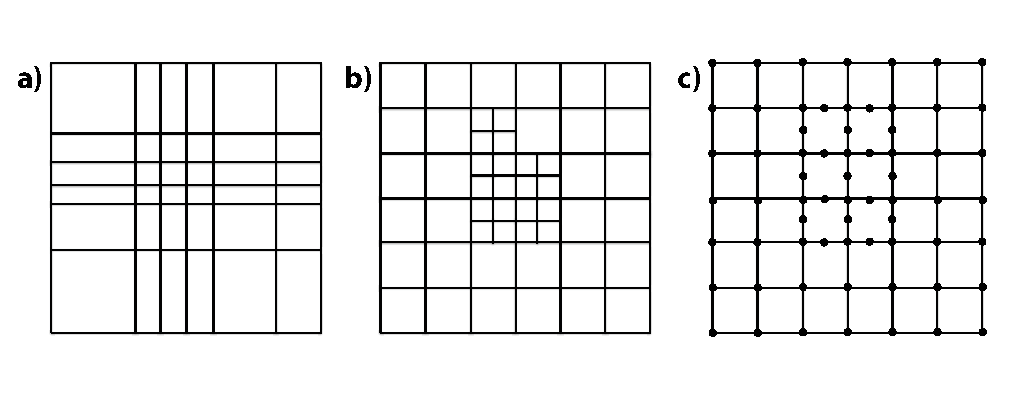
\includegraphics[width=\textwidth,height=\textheight,keepaspectratio]{Intro/refinement_types.eps}}
   \caption{Simplified examples of adaptive refinement techniques: (a) \emph{r}-refinement ---
    The number of grid cells is held constant, but the spacing between them changed,
    (b) \emph{h}-refinement --- the number of grid cells is increased by subdividing the grid, and
    (c) \emph{p}-refinement --- the polynomial order on the sub-grid scale is increased over the area of interest. The black
    dots represent the nodes in each grid cell.
   }
   \label{fig:refinetypes}
\end{figure}

   \subsubsection{r-refinement}
   In \emph{r}-refinement, the grid topology and number of grid elements remain unchanged;
instead, the elements are dynamically redistributed to increase resolution in parts of the grid 
while decreasing it everywhere else (Fig. \ref{fig:refinetypes}a). This dynamic mesh 
redistribution creates smoother transition regions between resolutions but
requires a complex global remapping of the mesh to move the location of the high 
resolution. The number of refined areas that can be formed are limited, and if the 
remapping transformation algorithms are not carefully constructed, grid tangling problems
and convergence issues can arise \citep{budd2009adaptivity}. \emph{r}-refinement is the 
dynamic version of static stretched grids.

In an early application of \emph{r}-refinement, \cite{Dietachmayer:1992sj} and 
\cite{dietachmayer1992application} used this global grid redistribution
technique to increase resolution in areas where the estimated solution
error is high. \cite{giraldo2000lagrange} and
\cite{iselin2002dynamic} applied this type of dynamic
adaptation for the 2D shallow water equations and advection problems,
respectively. More recently, \cite{Walsh:2010om} studied  
two-dimensional baroclinic instability with \emph{r}-refinement and
\cite{kuhnlein2012modelling} implemented \emph{r}-adaptivity within a 3D
Cartesian framework. \cite{bauer2014simulation} used \emph{r}-refinement grids guided by
error estimates in a shallow water model, and
\cite{weller2016mesh} demonstrated \emph{r}-refinement use on the
sphere.

   \subsubsection{h-refinement: Adaptive Mesh Refinement}
   Adaptive mesh refinement (AMR), also known as \emph{h}-refinement, increases resolution 
locally either by adding cells within the grid structure or by overlaying additional cells of finer 
resolution on top of the grid without changing the base grid structure (Fig. \ref{fig:refinetypes}b). 
Nested grids are the comparable static refinement technique.
            
\cite{skamarock1989adaptive} and
\cite{skamarock1993adaptive} implemented AMR by placing finer-resolution
meshes over the coarse grid in areas which had large truncation error
estimates. The grid-cell solutions and boundary conditions between the
finer-resolution meshes and the base grid are continually updated.  In
a more recent example,
\cite{Chen:2011kk} use AMR to overlay high-resolution meshes in areas
of interest in a shallow water model on a cubed-sphere grid.

Examples of AMR techniques which locally add and remove cells to the base
grid for the shallow water equations on the sphere have been presented
by
\cite{behrens2005amatos},
\cite{lauter2007parallel},
\cite{st2007comparison} and
\cite{marras2015simulation}.  Both
\cite{behrens2005amatos} and
\cite{lauter2007parallel} use conformal unstructured finite element
meshes.  In conformal grids, each cell shares an edge with exactly one
other cell, while in a non-conforming grid, cells can share an edge with
more than one neighboring element (Fig. \ref{fig:conform_noncon}).
Conformal grids can maintain conservation properties easily, avoid possible
discontinuities at refinement boundaries, and provide smoother transitions.
Non-conformal grids can provide more flexible refinement capabilities and, 
with simpler computational grid structures, run more efficiently on
large parallel supercomputers \citep{jablonowski2009block}.
The two AMR models described in
\cite{st2007comparison}, a block-structured finite-volume method on a
latitude-longitude grid and a spectral-element method on a cubed-sphere
grid, use nonconforming meshes and a quad-tree based AMR method with
gradient- or vorticity-based refinement criteria.
\cite{marras2015simulation} compared the use of an AMR approach on
several structured and unstructured non-conformal grids.  

\begin{figure}
   \centerline{%
   \noindent
   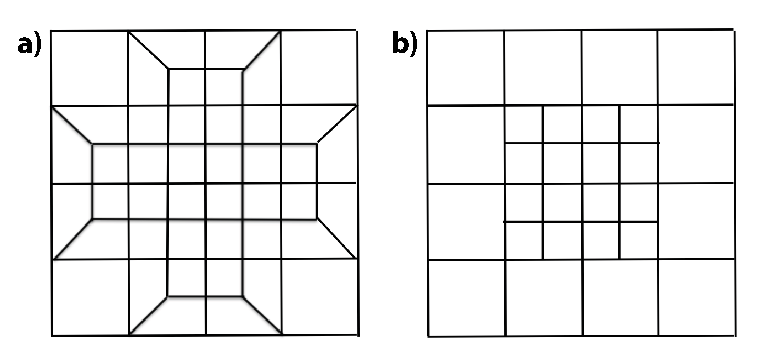
\includegraphics[width=\textwidth,height=\textheight,keepaspectratio]{Intro/mapping-conform.eps}}
   \caption{(a) Conformal grid --- each cell shares an edge with exactly one other cell and
    (b) Non-conformal grid --- cells can share an edge with more than one neighbor, 
    which results in hanging nodes.
   }
   \label{fig:conform_noncon}
\end{figure}

Use of AMR in a
regional model paired with a physical parameterization package was
presented in \cite{bacon2000dynamically}. OMEGA has been 
tested in forecasting hurricane storm tracks \citep{bacon2007hurricane}.
AMR methods have also been investigated for 
2D flow fields in Cartesian geometry. Recent examples include 
\cite{muller2013comparison} and \cite{kopera2014analysis} 
who analyzed a tree-structured AMR algorithm for 
non-hydrostatic dynamical cores in the x-z plane, and  
\cite{hendricks2016evaluation} who explored static and dynamic AMR for 
tropical-cyclone-like vortices in a shallow water model 
on an $f$-plane with a constant Coriolis parameter $f$.

   \subsubsection{p-refinement: Adaptive Order Refinement}
The third type of dynamic refinement, \emph{p}-refinement, holds the
grid spacing fixed but changes the order of the polynomial approximation
within each grid element to increase local resolution. Use of \emph{p}-refinement
with Discontinuous Galerkin (DG) methods for the shallow water equations
were described by \cite{kubatko2009dynamic} and
\cite{tumolo2015semi}. For smooth problems, \emph{p}-refinement offers a high rate of 
convergence with significantly less computational expense than other refinement types, 
but it has difficulty resolving sharp gradients in the flow field. To ameliorate these problems,
a hybrid refinement method that combines the
\emph{h}- and \emph{p}-refinements methods was demonstrated by
\cite{eskilsson2011hp}. \cite{blaise2012dynamic} used an \emph{hp}-adaptive DG method to model
the shallow water equations on a sphere for global tsunami
simulations and \cite{kopera2014analysis} implemented an DG method with \emph{hp}-refinement
in a two dimensional $xz$-projection of the compressible Euler equations.

\section{Challenges associated with dynamic refinement}
It has been nearly 30 years since the first adaptive atmospheric models 
were published \citep{skamarock1989adaptive,Dietachmayer:1992sj}.  Static refinement has been used for decades 
in regional weather models and VRGCMs have become a growing fixture in global climate modeling.  
Adaptive refinement for atmospheric modeling has remained mostly an academic exercise, 
with recent development centered on testing various refinement techniques in idealized one 
and two dimensional systems. Modeling the atmosphere is a far more complex problem 
than current applications of dynamic refinement as features of interest are more diverse and less 
well defined. To that end, there are several ongoing challenges that need to be addressed for AMR
to become a tool for climate and weather modeling. 

The key issue that most recent dynamical refinement work has been seeking to address is
the development of robust numerical methods that run efficiently on today's supercomputers.
A continuously changing grid structure sharply increases the difficulty in developing
numerical schemes that are efficient, accurate, and stable.
Dynamic refinement models still need to be locally conservative, preserve monotonicity, 
and minimize and manage numerical artifacts that arise from the grid refinement structure. 
Furthermore, any method must preserve consistency in the full equation sets. 
For example, at around 10 km resolution the hydrostatic approximation is no longer valid and models
need to solve the more complex full non-hydrostatic equations. 

Adaptive methods present more challenges for running simulations 
on current massively parallel supercomputers than traditional
static models face.  The processor and memory requirements of a dynamic refinement 
model change as grid elements are added and removed. Dynamic refinement techniques 
also use complex data structures requiring more computational overhead to organize
the grid elements and communicate the grid changes.
For dynamic refinement methods to become more 
mainstream, they need to be more computationally efficient than current uniform models yet generate the same accuracy and skill. 
Both the block-structured \citep{jablonowski2009block,Chen:2011kk} and unstructured quad-tree refinements \citep{lauter2007parallel,blaise2012dynamic} show promise as methods that ensure computationally efficient refinement on high performance computing platforms.

Another issue facing both dynamic and static VRGCMs is scale-aware physics parameterizations. 
In current uniform climate and weather models, the physics schemes that approximate the
unresolved and sub-grid scale processes are specifically tuned to the model's resolution. 
Increasing resolution without re-tuning the physics parameterizations can adversely affect
results \citep{rauscher2013exploring,zarzycki2014aquaplanet}. So, in adaptive schemes, 
the sub-grid parameterizations need to be able to adjust for changes in scale.  
A model would need to be able to phase out certain sub-grid processes, like deep
convection, as resolution is increased and these processes are resolved on the actual mesh.
Several parameterization schemes (e.g. the newly developed cloud scheme 
Cloud Layers Unified By Binormals (CLUBB) in the National Center for Atmospheric Research's
Community Atmosphere Model) are being designed to work with varying vertical and horizontal resolutions.

A final issue in dynamic refinement is the selection of refinement criteria that determine where refinement is added.
If a refinement criterion is too selective, key features will not be refined; if a criterion is too relaxed, 
refinement areas will become too large, making the model inefficient. Furthermore, the multiscale nature 
of the atmosphere and its interconnectivity creates a plethora of refinement criteria possibilities 
such that one set of criteria will not work effectively on all possible features of interest. Thus finding criteria 
that detect the areas that need to be refined as accurately and efficiently as possible is vital for 
effective implementation of adaptive meshes. A variety of criteria have been proposed and tested
in the literature including local error estimates 
\citep{skamarock1989adaptive,lauter2007parallel,bauer2014simulation} and physical
variables like pressure or wind \citep{bacon2000dynamically,st2007comparison,kopera2014analysis}.

Global dynamic refinement models retain potential as powerful tools for 
solving complex, nonlinear, multiscaled weather and climate systems.  
 Dynamic refinement could benefit many applications involving transient 
localized phenomena including tropical cyclones, atmospheric blocking events, orographic 
precipitation, and pollution dispersion. Even long-term climate simulations could benefit as 
localized flow structures may be important in determining climate signals, such as modeling
atmospheric rivers on the West coast of the United States.  

\section{Outline of Thesis}
This thesis presents ongoing work to implement AMR within 
a new nonhydrostatic, finite-volume dycore and to demonstrate 
AMR's effectiveness in improving model accuracy and 
resolving multiscale features. These efforts are accomplished by 
implementing a hierarchy of new and existing test cases of increasing 
complexity for the 2D shallow water and 3D non-hydrostatic equations. 
The thesis is organized as follows. In Chapter \ref{chap:basicsw} we implement existing 
shallow water test cases and develop several new ones to assess 
the capabilities of AMR in the shallow water version of the 
\cite{mccorquodale2015adaptive} finite volume Chombo AMR 
model. The results of this research were published in \cite{ferguson2016analyzing}.
Chapter \ref{chap:forcedsw} presents two different 
forced shallow water systems with moisture variables designed to 
represent convective and precipitation processes as more challenging 
testbeds to use with the finite volume Chombo AMR model. In 
Chapter \ref{chap:3dmodel}, we investigate the effects of AMR using 
the 3D non-hydrostatic version of the finite-volume Chombo AMR model in 
two 3D test cases. The first consists of a simple dry flow without 
forcing while the second adds a simplified physics parameterization 
scheme. Conclusions and future directions are presented in Chapter \ref{chap:conclusion}.